% 默认页面大小 4:3
\documentclass[10pt]{beamer}
% 页面大小 16:10
% \documentclass[10pt, aspectratio=1610]{beamer}
% 页面大小 16:9
% \documentclass[10pt, aspectratio=169]{beamer}
% 页面大小 14:9
% \documentclass[10pt, aspectratio=149]{beamer}
% 页面大小 1.41:1
% \documentclass[10pt, aspectratio=141]{beamer}
% 页面大小 5:4
% \documentclass[10pt, aspectratio=54]{beamer}
% 页面大小 3:2
% \documentclass[10pt, aspectratio=32]{beamer}

\usetheme[logo=UCAS, sublogo=AMSS]{ucas}
% logo 的选项: CAS, UCAS
% sublogo 的选项: AMSS, AMSS2018, UCAS

\usepackage[backend=biber, citestyle=authoryear]{biblatex}

% 具有字形变化的字母编码工具包,若不需要,可注释或删除,
% \usepackage[T1]{fontenc}
% 引入 [T1]{fontenc] 工具包在低版本 TeX 编译环境可能因为某些字符,如`~' 导致编译失败,以下命令可解决问题
% \DeclareTextCommand{\nobreakspace}{T1}{\leavevmode\nobreak\ }

% 用于超文本链接的工具包
\usepackage{hyperref}

\usepackage{amsmath}
\usepackage{amsfonts}
\usepackage{amssymb}

\usepackage{graphicx}
\usepackage{subfigure}

\usepackage{tikz}
\usetikzlibrary{shapes.geometric, arrows}

\newcommand{\fn}{\normalsize}
\newcommand{\ff}{\footnotesize}
\newcommand{\fs}{\scriptsize}
\newcommand{\ft}{\tiny}

% 引入参考文献列表的 .bib 文件
\addbibresource{ref.bib}

\subtitle[TBM掘进机近前方岩体构造的精细刻画与分布参数预测]{TBM掘进机近前方岩体构造的精细刻画与分布参数预测}
\title[毕业设计]{毕业设计}
\author[李泉彰]{李泉彰}
\institute[中国科学院大学~~数学科学学院]{中国科学院大学~~数学科学学院}
\date[\today]{\today, 中国北京}
\subject{展示主题}
\keywords{TBM,岩体节理 | 裂隙构造,扁平椭球参数化,混合 ARIMA,样本可视化}

\begin{document}

\begin{frame}[plain]
  \maketitle
\end{frame}

\begin{frame}[t]
  \frametitle{目录}
  \tableofcontents
\end{frame}

\section[Introduction]{引言}\label{sec:1}
\subsection[Background]{背景}\label{subsec:1-1}

\fs{
\begin{frame}{背景}

\begin{columns}

    \column{.4\textwidth}
    \ff
    {
        \alert{TBM(tunnel boring machine)}\\
        \begin{enumerate}
            \item \structure{功能} 隧道掘进
            \item \structure{用途} 公路铁路工程、水利水电设施、市政工程建设
            \item \structure{困难} 缺乏有效预测近前方岩体力学参数的手段。而岩体的力学参数可以根据岩体的结构、利用高阶多尺度算法得到。因此问题归结为如何预测近前方岩体结构。
        \end{enumerate}
    }
    
    \column{.5\textwidth}
    \begin{figure}
        \centering
        % Requires \usepackage{graphicx}
        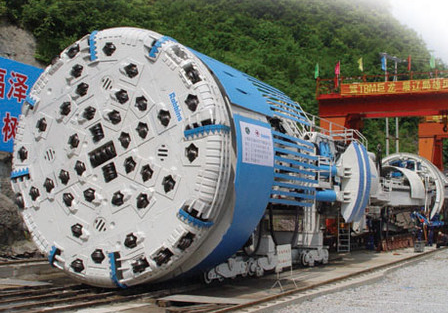
\includegraphics[width=5cm]{figure/TBM.png}
    \end{figure}

\end{columns}

\end{frame}

\subsection[Model]{模型提出}\label{subsec:1-2}
\begin{frame}{模型提出}
\begin{columns}
    \column{.5\textwidth}
        \fs
        {
            \structure{岩体抽样化} \cite{hudson1979discontinuities} 提出岩体的力学行为由岩体裂隙(包括:接缝,裂隙和微裂隙等)的几何参数所决定,而岩体裂隙又可以抽象为扁平的椭球(忽略厚度后可以认为是椭圆)。抽象后的岩体如右图。\\
            在特定采样段,岩体中裂隙的分布就由椭球的九个参数(如下表)满足的概率分布所决定。
        
            \begin{table}[b]
                \centering
                \begin{tabular}{cccc}
                \toprule
                    三个轴长度 & $S_x$ & $S_y$ & $S_z$ \\
                    \midrule
                    三个角度 & $\theta_x$ & $\theta_y$ & $\theta_z$ \\
                    \midrule
                    中心点坐标 & $X$ & $Y$ & $Z$\\ \bottomrule
                \end{tabular}
                \caption{椭球参数表}
                \label{tab:parameters}
            \end{table}
        }
        
    \column{.5\textwidth}
    \begin{figure}
        \centering
        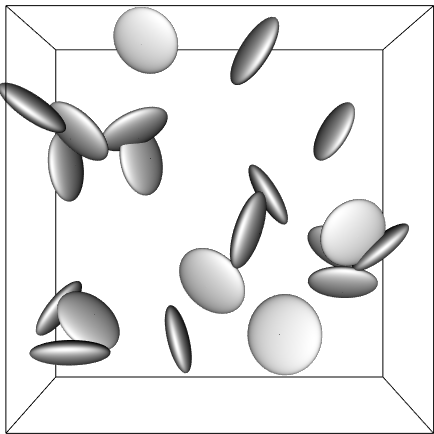
\includegraphics[width=5cm]{figure/abstract.png}
        \caption{岩体抽象}
        \label{fig:abstract}
    \end{figure}
\end{columns}

\end{frame}

\begin{frame}{模型提出}
\fs{
    \alert{基本假设} 假设这九个概率分布独立同分布的,因此可以分开预测,以下仅以参数$S_x$为例。

	\begin{enumerate}
		\item 根据已有时刻$(t = 1, 2, 3, \dots, T)$的椭球样本拟合$S_x$所满足的分布,并且得到每一个时刻分布的参数向量$(\hat{p}_1(1),~ \hat{p}_2(1),~  \dots),$~~ $(\hat{p}_1(2),~ \hat{p}_2(2),~ \dots),$~~ $\dots,$~~ $(\hat{p}_1(T),~ \hat{p}_2(T),~ \dots)$。
		\item 以分布的第一个参数$p_1$为例,它在不同时刻的取值$p_1(t)$构成时间序列。通过的\cite{zhang2003time}所提到的混合ARIMA模型,可以将其拆解为线性部分和非线性部分,即$p_1(t) = L(t) + N(t)$。
		\item 利用第一步所得到的$p_1(t)$的一个抽样${\hat{p}_1(1), \hat{p}_1(2), \dots, \hat{p}_1(T)}$来拟合出$\hat{L}(t)$和$\hat{N}(t)$。
		\item 利用$\hat{L}(t)$和$\hat{N}(t)$得到下一时刻$p_1$的预测值$\hat{L}(T+1)+  \hat{N}(T+1)$。
		\item 重复上述程序可以得到下一个时刻椭球的九个参数所满足的分布以及分布的参数,并且不同时刻椭球的密度${density(1), density(2), \dots, density(t)}$也可看做一个时间序列,利用之前的步骤也就可以得到$T+1$时刻椭圆密度的估计$\hat{d}(T+1)$。
		\item 根据预测得到的九个分布函数和椭圆密度,利用特定的抽样方法,在下一时刻岩体所在的统计窗内抽取裂隙并进行可视化。
	\end{enumerate}
}
\end{frame}
}

\begin{frame}{模型简述}
\fs{
	\alert{问题} 预测TBM近前方椭球的九个参数满足的概率分布函数以及椭球的密度(单位体积椭球中心点的个数)。\\
	\alert{基本假设} 假设这九个概率分布独立同分布的,因此可以分开预测,以下仅以参数$S_x$为例叙述。\\
	\alert{模型简述:}
	\begin{enumerate}
	\item 根据已有时刻$(t = 1, 2, 3, \dots, T)$的椭球样本拟合$S_x$在相应采样段所满足的分布以及分布的参数向量$(\hat{p}_1(T),~ \hat{p}_2(T),~ \dots)$。
	\item 根据分布的参数向量的分量在不同采样段的取值构建和拟合其满足的时间序列模型。
	\item 用前两步中的模型预测TBM近前方$S_x$满足的分布类型和分布的参数向量,以此作为$S_x$的分布函数的预测。
	\end{enumerate}	 
}
\end{frame}

\section[Estimation of Distribution]{分布拟合}\label{sec:2}
\subsection[Length]{长度参数}\label{sec:2-1}
\begin{frame}{长度参数}
    对于椭球的九个参数,与长度有关的三个参数${S_x, S_y, S_z}$可以看作一类。\cite{warburton1980stereological}中提到,工程实际应用中这三个参数通常来自于指数分布族(公式(\ref{equ:exp}))或者对数正态分布族(公式(\ref{equ:LogNorm}))。
    \begin{equation}\label{equ:exp}
    	% \adddotsbeforeeqnnum
    	f(x, \lambda) = \lambda\exp(-\lambda x), \quad x > 0
    \end{equation}
    
    \begin{equation}\label{equ:LogNorm}
    	% \adddotsbeforeeqnnum
    	f(x, \mu, \theta) = \frac{1}{\sqrt{2\pi}\sigma}\exp(-\frac{1}{2\sigma^2}(\ln x - \mu)^2), \quad x > 0
    \end{equation}
\end{frame}

\begin{frame}
\fs{
    	这两种分布都有可能是椭球长度的参数符合的分布,本文利用了Kolmogorov-Smirnov检验统计量在两种分布之间的选取更符合实际情况的分布。\\
   		\alert{以$S_x$为例具体流程如下:}
	\begin{itemize}
		\item 首先假设样本$S_x$符合对数正态分布函数Log-N$(\mu, \sigma^2)$。利用我们已有的样本$\{X_1, X_2, \dots, X_n\}$计算出正态分布参数的矩估计得到$\log(L_x) \sim {\rm N}(\hat{\mu}, \hat{\sigma}^2)$。进而利用\cite{page1977approximations}介绍的逼近正态分布分布函数的方法得到逼近分布函数$F_{lognormal}(x)$。
		\item 第二步假设样本$S_x$符合指数分布函数${\rm Exp}(\lambda)$,同样利用矩估计得到分布函数$F_{exponential}(x)$。
		\item 第三步根据样本$\{X_1, X_2, \dots, X_n\}$构造阶跃函数(其它的非参数方法得到的分布也可):
		\begin{equation}
			F_n(x) = \frac{1}{n}\sum_{i = 1}^{n}I_{[-\infty, x]}(X_i)
		\end{equation}
		\item 最后分别将$F_{lognormal}$和$F_{exponential}$带入公式
		\begin{equation}\label{equ:KS}
		D = \sup_x|F_n(x) - F(x)|	
		\end{equation}
		的$F(x)$中,算出两个$D$值,使得$D$值较小的分布就作为样本的分布函数,相对应的概率密度函数也就可以作为样本分布的概率密度函数。
	\end{itemize}
}
\end{frame}

\subsection[Angle]{角度参数}\label{2-2}
\begin{frame}{角度参数}
\fs{
	因为椭球可以进一步简化为扁平的椭圆,椭球的三个角度参数则转化为该椭圆的法线方向在球面坐标系(如下图)中的两个参数$(\varphi, \theta)$和椭圆在所在平面内旋转的角度$\gamma$(指的是旋转方向与X轴的夹角)。\\

为了更好地描述这三个参数,我们采用Fisher分布\footcite{fisher1953dispersion}\\

Fisher分布描述的是集中于空间或平面内某个角附近随机分布的角,由集中角度和集中程度$\kappa$两个参数决定,$\kappa$越大集中程度越高。\footnote{\fs{$(\varphi, \theta)$用三维空间Fisher分布,$\gamma$用二维平面的Fisher分布}}\\

公式(\ref{equ:fisher})是二维Fisher分布的表达式。集中角度为$\theta_0$,集中程度为$\kappa$
}


\begin{equation}\label{equ:fisher}
	%\adddotsbeforeeqnnum
	\mathrm{d}f(\theta) = \frac{\kappa}{2\sinh\kappa}\exp(\kappa\cos(\theta - \theta_0))\sin(\theta - \theta_0)\mathrm{d}\theta
\end{equation}

\begin{columns}
    \column{.3\textwidth}
    \begin{figure}[!htbp]
    	\centering
    	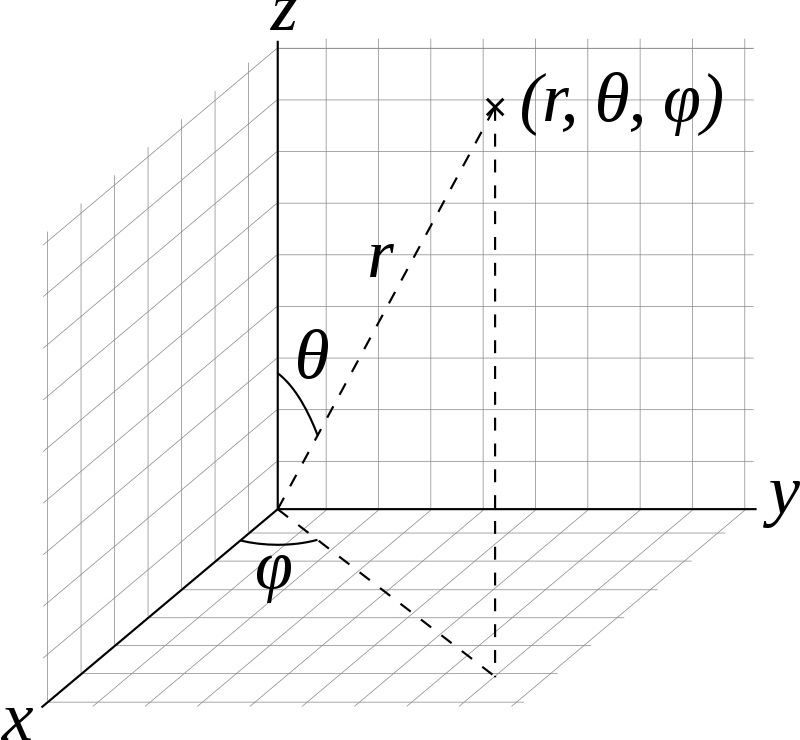
\includegraphics[width=2.5cm]{figure/Spherical}
    	\caption{球面坐标系}
    	\label{fig:Spherical}
    \end{figure}
    \column{.3\textwidth}
      \begin{figure}[!htbp]
		\centering
			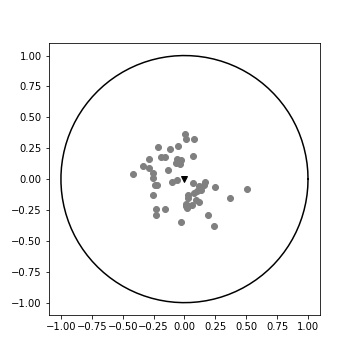
\includegraphics[width=2.5cm]{figure/fisher_k30}
			\caption{Fisher分布$\kappa = 30$}
			\label{fig:fisher_k30}
    	\end{figure}
    	
    \column{.3\textwidth}
      \begin{figure}[!htbp]
		\centering
			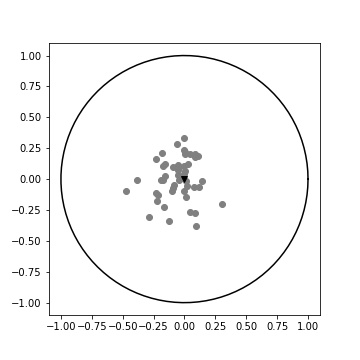
\includegraphics[width=2.5cm]{figure/fisher_k300}
			\caption{Fisher分布$\kappa = 300$}
			\label{fig:fisher_k300}
    	\end{figure}
\end{columns}
	
\end{frame}

\subsection[Location]{位置参数}\label{subsec:2-3}
\begin{frame}{位置参数}
\ff{
	与位置有关的三个参数${X, Y, Z}$没有已知的常见分布形式,但是考虑到岩体力学行为的各向同性,均匀分布可以作为一个合理的选择。另外正态分布也可以作为备选分布。接下来利用选取长度参数分布的步骤在这二者中选取合理的分布即可。

	\alert{Remark:}
	在实际工程项目中,椭圆参数的分布可能并不唯一,例如椭圆的长度参数$S_x$可能在不同的局部取样段符合不同的分布类型,在这种情况下,我们可以选取出现较多的分布类型作为全局最优的分布类型。
}
\end{frame}

\subsection[Sample]{分布拟合算例}\label{subsec:2-4}
\begin{frame}{分布拟合算例}

\ff{
	通过数值算例检验\cite{fisher1953dispersion}提到的Fisher分布参数的估计方法。

	对于二维平面的Fisher分布,考虑到二维平面角度关于原点的对称性,我们只需要对集中角度$\gamma = 0$的情况检验即可。

	分别对$\kappa = 20, 40, \dots, 300$的情况抽取$30$和$300$个样本,对这30组数据每一组重复$50$次,将拟合结果平均得出$\gamma$和$\kappa$的估计值$\hat{\gamma}$和$\hat{\kappa}$。具体拟合结果如下图

	\begin{columns}
	\column{.5\textwidth}
		\begin{figure}
		\centering
		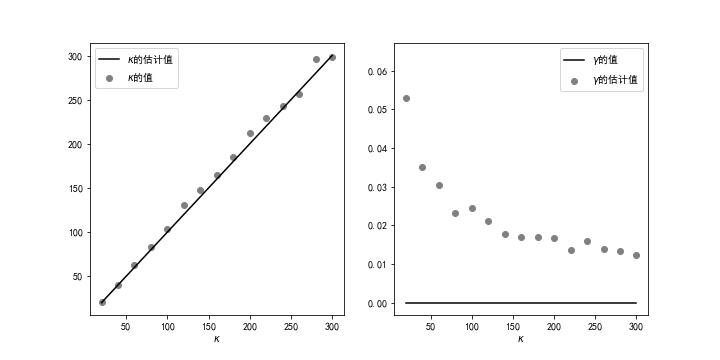
\includegraphics[width=5cm]{figure/EstFisherN30}
		\label{fig:EstFisherN30}
		\caption{Fisher分布的拟合(样本数等于30)}
		\end{figure}%
	
	\column{.5\textwidth}
		\begin{figure}
		\centering
		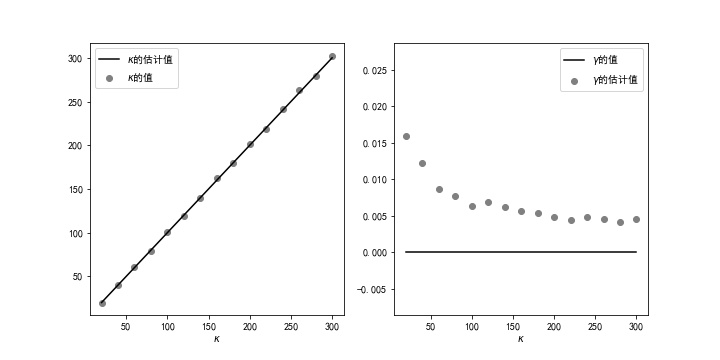
\includegraphics[width=5cm]{figure/EstFisherN300}
		\label{fig:EstFisherN300}
		\caption{Fisher分布的拟合(样本数等于300)}
		\end{figure}
	\end{columns}
}
\end{frame}

\section[Time Series]{时间序列预测}\label{sec:3}

\subsection[Modle]{时间序列模型}\label{subsec:3-1}

\begin{frame}
\ff{
	将所有采样段得到的$S_x$的分布的参数的第一个分量$\hat{\mu}_t( = X_t)$放在一起(其余分量同理),可以看作是一组取之于时间$t$的时间序列$\{X_1, X_2, \dots, X_T\}$的一个样本。而该时间序列可以看作如下数学模型\footcite{de1992some}:
\begin{equation}\label{TimeseriesModle}
	X_t = h(X_{t-1}, X_{t-2}, \dots, X_{t-p}, \epsilon_{t-1}, \epsilon_{t-2}, \dots, \epsilon_{t-q}) + \epsilon_{t}
\end{equation}
的一个抽样。其中$\{\epsilon_{t}\}$是一组独立同分布、有着共同均值$\mu$和共同方差$\sigma$的白噪声,一般而言,将样本数据中心化以后可以认为白噪声的均值$\mu = 0$。

\alert{目标:}根据$\{X_1, X_2, \dots, X_T\}$得到上式中$p$、$q$的估计,$h$的表达式的估计,和白噪声方差$\sigma$的估计。
}	
\end{frame}

\begin{frame}{ARIMA模型}
\ff{
	根据\cite{zhang2003time}的文献,我们可以分别用不同的模型来近似$h$的线性部分和非线性部分。$h$线性部分可以用ARIMA模型\footcite{box1994time}来近似:
	
	\begin{equation}\label{equ:ARIMA}
	LX_t + \sum_{i=1}^{p}\Phi_iX_{t-i} = \mu + \epsilon_t + \sum_{j=1}^{q}\theta_j\epsilon_{t-j}
	\end{equation}
	
	该模型的训练分为如下几个部分:
	\begin{enumerate}
	\item 数据平稳化:通常我们根据自相关系数趋于零的速度来判断数据的平稳性,如果数据是非平稳的,则通过差分将数据平稳化(一般差分的次数不超过两次)。
	\item 模型选择:根据\cite{box1994time},数据的自相关系数和偏自相关系数可以用于模型中参数$p$和$q$的选择。
	\item 参数拟合:选择了特定$p$和$q$以后,对$\Phi_i$、$\theta_j$、$\mu$的选择相当于利用非线性优化方法最小化预测值与真实值的误差
	\item 模型评估:我们可以事先留出部分数据作为验证集,利用白噪声检验,判断模型在验证集上的预测值与真实值之间的差是否是独立同分布的正态分布。如果没通过就返回第二步重新选取$p$和$q$,然后进行步骤三四。
\end{enumerate}
	
	如果数据具有周期性也可以添加上周期项使用季节性ARIMA模型。
}
\end{frame}

\begin{frame}{神经网络模型}
\ff{
	\cite{zhang2003time}提到利用人工神经网络ANN模型(公式(\ref{equ:ANN}))来近似非线性部分效果会很好。
	\begin{equation}\label{equ:ANN}
		y_t = \alpha_0 + \sum_{j = 1}^{q}\alpha_jg(\beta_{0j} + \sum_{i = 1}^{p}\beta_{ij}y_{t-i}) + \epsilon_t
	\end{equation}
	其中函数$g(x)$被称作激活函数,通常被取做logistic函数(公式(\ref{equ:logistic})),当然双曲正切函数$g(x) = a\tanh(bx)$或其他可行的函数也可以替代。
	\begin{equation}\label{equ:logistic}
		g(x) = \frac{1}{1 + \exp(-x)}
	\end{equation}
	
	真实值与ARMIA模型的预测值之间的误差可以作为神经网络模型的训练数据,模型的具体的训练步骤与ARIMA模型的第二到第四步类似,只不过第三步中对于表达式系数的预测一般可以用误差逆传播法、遗传算法\cite{montana1989training}......
}
\end{frame}

\begin{frame}{模型训练}
\ff{
	实际应用中,对于ARIMA模型的训练利用的是Python的库\textit{pmdarima},它是专门用来求解拟合ARIMA模型以及SARIMA模型的库,利用函数\textit{auto\_arima}可以便利地求出在当$p$和$q$限制在一定范围内时最优的$p$和$q$的估计值以及ARIMA模型相应系数。对于ANN模型的构建则使用的是\textit{keras}库,它相当于是一个神经网络API,有着用户友好、模块化程度高、扩展性好等优点,可以以\textit{TensorFlow}作为后端运行,速度也较快。
}
\end{frame}

\subsection[Sample]{时间序列算例}
\begin{frame}{时间序列算例}
\ff{
	我们选取澳大利亚的月啤酒生产量作为时间序列样本,下图反映出该序列有很强的季节性,波动规律大约是以一年为周期,因此我们采用季节性ARIMA模型与ANN模型的混合模型来进行预测。
	\begin{figure}[!htbp]
		\centering
		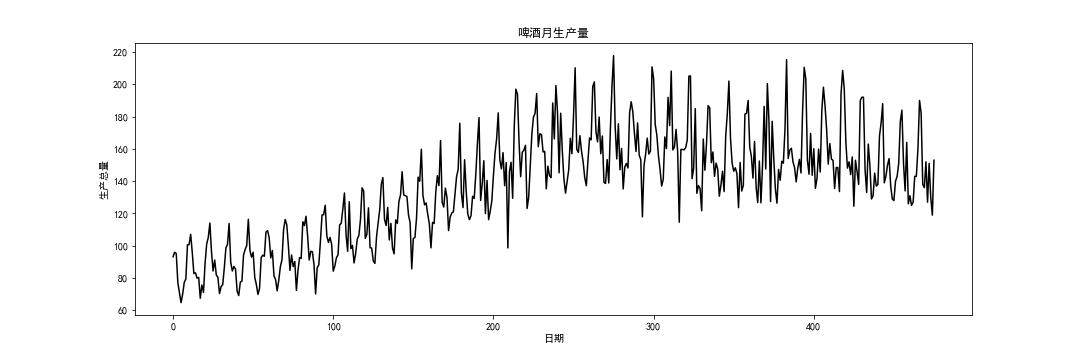
\includegraphics[width=5cm]{figure/monthly_beer_production}
		\caption{啤酒月生产量}
		\label{fig:monthly_beer_production}
	\end{figure}
	调用\textit{auto\_arima}函数,拟合得到最接近的模型为SARIMA$(3, 1, 3)\times(2, 0, 1, 12)$(即周期确实为$12$个月)。对于该种季节性数据,我们的混合的结果如下图\ref{fig:predictions3}。
	\begin{figure}[!htbp]
		\centering
		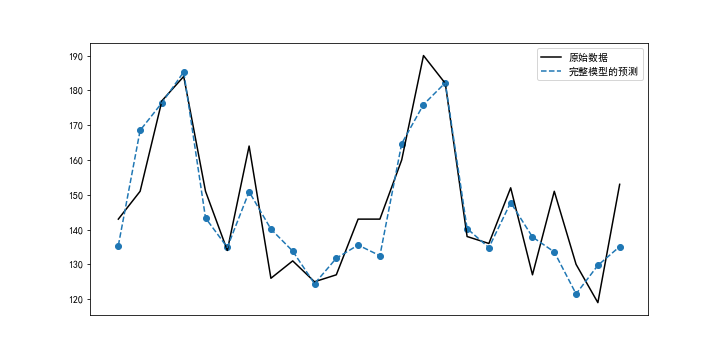
\includegraphics[width=5cm]{figure/predictions3}
		\caption{啤酒月生产量预测}
		\label{fig:predictions3}
	\end{figure}
	可以看到在验证集上我们的模型基本上很好拟合了实际数据。
}
\end{frame}


\section[Sampling And Visualization]{抽样与可视化}\label{sec:4}

\subsection[Sampling]{抽样}\label{subsec:4-1}
\begin{frame}{抽样}

\ff{
	通过前文所述的方法,根据掘进机已经驶过的区域的椭球的数据,可预测掘进机近前方区域椭球九个参数可能的分布和近前方断层的密度$\hat{d}(T+1)$。进而,对于一个尺寸为$a \times b \times c$(${\rm m}^3$)的矩形统计窗,我们可以基于预测出的这些分布的性质,抽取出$a \times b \times c \times \hat{d}(T+1)$个样本,并将其组成$a \times b \times c \times \hat{d}(T+1)$个椭球,来作为TBM近前方岩体的裂隙的分布。\\
	
	对于均匀分布、对数正态分布、指数分布的抽取,我们利用Python的\textit{random}库,该库内置了这些常见分布的随机数生成器。对于Fisher分布的抽取我们就利用近似公式\footcite{priest2012discontinuity}:
\begin{equation}\label{equ:FisherSample}
\theta - \theta_i = \Delta(\theta) = \cos^{-1}[\frac{\ln(1 - {\rm Random}(0, 1))}{\kappa}+1]
\end{equation}


}

\end{frame}

\subsection[Visualization]{可视化}\label{subsec:4-2}
\begin{frame}{可视化}

\ff{
	\alert{使用工具}对于数据的可视化我们采用免费的开源软件VTK(Visualization Toolkit,即可视化工具包)。VTK封装了很多可视化过程中常用的数据结构和算法,其中就包括椭球绘制的算法\textit{vtkParametricEllipsoid}
	
	
	\alert{绘制流程\footcite{schroeder2000visualizing, avila2010vtk}:}\\
	\begin{columns}
	\column{.5\textwidth}
	$\quad$
	\structure{步骤一:}设置椭球参数\\
	\tikzstyle{process} = [rectangle,rounded corners, minimum width=2cm,minimum height=0.5cm,text centered, draw=black,fill=gray!30]
	\tikzstyle{arrow} = [thick,->,>=stealth]

	$\quad$
	\begin{tikzpicture}[node distance=2cm]
	\node (process1) [process] {vtkParametricEllipsoid};
	\node (process2) [process, below of=process1, yshift=1cm] {vtkPolyDataMapper};
	\node (process3) [process, below of=process2, yshift=1cm] {vtkActor};
	%\node (process4) [process, below of=process3, yshift=2cm] {vtkRenderer};
	%\node (process5) [process, left of=process4, xshift=4cm] {vtkRenderWindow};

	\draw [arrow] (process1) -- (process2);
	\draw [arrow] (process2) -- (process3);
	%\draw [arrow] (process3) -- (process4);
	%\draw [arrow] (process4) -- (process5);
	\end{tikzpicture}
	
	
	\column{.5\textwidth}
	$\quad$
	\structure{步骤二:}渲染椭球\\
	\tikzstyle{process} = [rectangle,rounded corners, minimum width=2cm,minimum height=0.5cm,text centered, draw=black,fill=gray!30]
	\tikzstyle{arrow} = [thick,->,>=stealth]
	$\quad$
	\begin{tikzpicture}[node distance=2cm]
	\node (process3) [process] {vtkActor};
	\node (process4) [process, below of=process3, yshift=1cm] {vtkRenderer};
	\node (process5) [process, below of=process4, yshift=1cm] {vtkRenderWindow};

	\draw [arrow] (process3) -- (process4);
	\draw [arrow] (process4) -- (process5);
	\end{tikzpicture}\\
	
	\end{columns}
}
	
\end{frame}

\begin{frame}{样例}
	\ff{
		
	\begin{table}[!htbp]
	\caption{椭球参数分布和密度}
	\label{tab:EiilpDisDensity}
	\centering
	\footnotesize% fontsize
	\setlength{\tabcolsep}{4pt}% column separation
	\renewcommand{\arraystretch}{1.2}%row space 
	\begin{tabular}{lcccccccc}
		\hline
		椭球参数 & \multicolumn{4}{c}{不同采样段椭球参数的分布}\\
		\cline{2-5}% partial hline from column i to column j
		\hline
		& 一 & 二 & 三 & 四 \\
		$S_x$ & Exp$(0.1)$ & Exp$(0.1)$ & Exp$(0.1)$ & Log-N$(2, 4)$\\
		$S_y$ & Exp$(0.1)$ & Exp$(0.1)$ & Exp$(0.1)$ & Log-N$(2, 4)$\\
		$S_z$ & Exp$(1)$ & Exp$(1)$ & Exp$(1)$ & Log-N$(0.6, 2)$\\
		$\gamma$ & Fisher$(10)$ & Fisher$(10)$ & Fisher$(10)$ & Fisher$(10)$\\
		$\theta$ & Fisher$(10)$ & Fisher$(10)$ & Fisher$(100)$ & Fisher$(10)$\\
		样本数 & $20$ & $40$ & $20$ & $20$\\	 
		\hline
	\end{tabular}
\end{table}

}
\end{frame}

\begin{frame}{样例}
	\ff{
		\begin{figure}
		\centering
		\begin{subfigure}{样例一}
			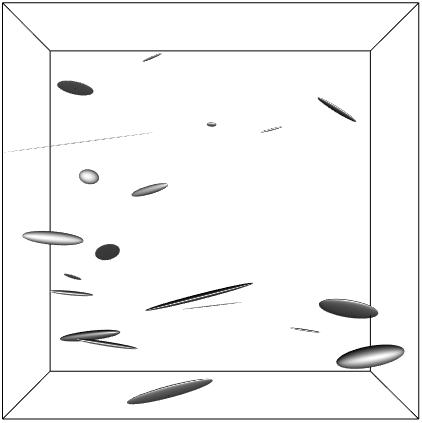
\includegraphics[width=2.5cm]{figure/visual1}
			\label{fig:visual1}
		\end{subfigure}
		~
		\begin{subfigure}{样例二}
			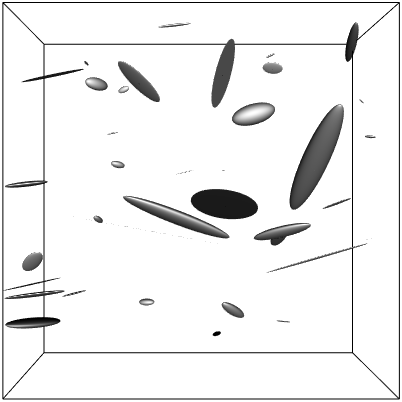
\includegraphics[width=2.5cm]{figure/visual2}
			\label{fig:visual2}
		\end{subfigure}
		\\
		\begin{subfigure}{样例三}
			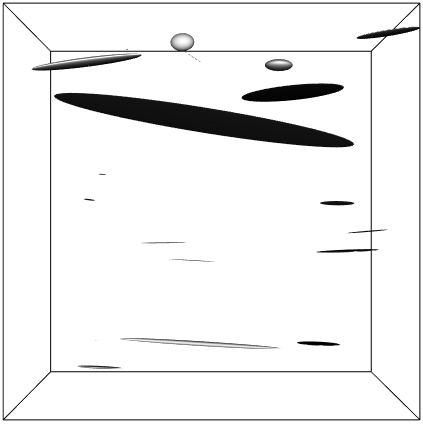
\includegraphics[width=2.5cm]{figure/visual3}
			\label{fig:visual3}
		\end{subfigure}
		~
		\begin{subfigure}{样例四}
			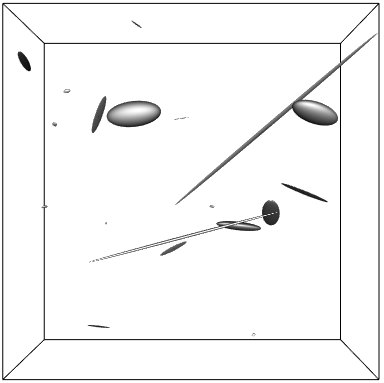
\includegraphics[width=2.5cm]{figure/visual4}
			\label{fig:visual4}
		\end{subfigure}
	\end{figure}
}
\end{frame}


\makeatother

\begin{frame}[noframenumbering, allowframebreaks, t]
  \frametitle{参考文献}
  \nocite{*}% 打印未引用,但已列入 .bib 文件内的文献
  \printbibliography%
\end{frame}

\begin{frame}[plain]
  \vfill
  \centerline{\Huge 谢谢!}
  \vfill
\end{frame}

\end{document}
